\documentclass[1p]{elsarticle_modified}
%\bibliographystyle{elsarticle-num}

%\usepackage[colorlinks]{hyperref}
%\usepackage{abbrmath_seonhwa} %\Abb, \Ascr, \Acal ,\Abf, \Afrak
\usepackage{amsfonts}
\usepackage{amssymb}
\usepackage{amsmath}
\usepackage{amsthm}
\usepackage{scalefnt}
\usepackage{amsbsy}
\usepackage{kotex}
\usepackage{caption}
\usepackage{subfig}
\usepackage{color}
\usepackage{graphicx}
\usepackage{xcolor} %% white, black, red, green, blue, cyan, magenta, yellow
\usepackage{float}
\usepackage{setspace}
\usepackage{hyperref}

\usepackage{tikz}
\usetikzlibrary{arrows}

\usepackage{multirow}
\usepackage{array} % fixed length table
\usepackage{hhline}

%%%%%%%%%%%%%%%%%%%%%
\makeatletter
\renewcommand*\env@matrix[1][\arraystretch]{%
	\edef\arraystretch{#1}%
	\hskip -\arraycolsep
	\let\@ifnextchar\new@ifnextchar
	\array{*\c@MaxMatrixCols c}}
\makeatother %https://tex.stackexchange.com/questions/14071/how-can-i-increase-the-line-spacing-in-a-matrix
%%%%%%%%%%%%%%%

\usepackage[normalem]{ulem}

\newcommand{\msout}[1]{\ifmmode\text{\sout{\ensuremath{#1}}}\else\sout{#1}\fi}
%SOURCE: \msout is \stkout macro in https://tex.stackexchange.com/questions/20609/strikeout-in-math-mode

\newcommand{\cancel}[1]{
	\ifmmode
	{\color{red}\msout{#1}}
	\else
	{\color{red}\sout{#1}}
	\fi
}

\newcommand{\add}[1]{
	{\color{blue}\uwave{#1}}
}

\newcommand{\replace}[2]{
	\ifmmode
	{\color{red}\msout{#1}}{\color{blue}\uwave{#2}}
	\else
	{\color{red}\sout{#1}}{\color{blue}\uwave{#2}}
	\fi
}

\newcommand{\Sol}{\mathcal{S}} %segment
\newcommand{\D}{D} %diagram
\newcommand{\A}{\mathcal{A}} %arc


%%%%%%%%%%%%%%%%%%%%%%%%%%%%%5 test

\def\sl{\operatorname{\textup{SL}}(2,\Cbb)}
\def\psl{\operatorname{\textup{PSL}}(2,\Cbb)}
\def\quan{\mkern 1mu \triangleright \mkern 1mu}

\theoremstyle{definition}
\newtheorem{thm}{Theorem}[section]
\newtheorem{prop}[thm]{Proposition}
\newtheorem{lem}[thm]{Lemma}
\newtheorem{ques}[thm]{Question}
\newtheorem{cor}[thm]{Corollary}
\newtheorem{defn}[thm]{Definition}
\newtheorem{exam}[thm]{Example}
\newtheorem{rmk}[thm]{Remark}
\newtheorem{alg}[thm]{Algorithm}

\newcommand{\I}{\sqrt{-1}}
\begin{document}

%\begin{frontmatter}
%
%\title{Boundary parabolic representations of knots up to 8 crossings}
%
%%% Group authors per affiliation:
%\author{Yunhi Cho} 
%\address{Department of Mathematics, University of Seoul, Seoul, Korea}
%\ead{yhcho@uos.ac.kr}
%
%
%\author{Seonhwa Kim} %\fnref{s_kim}}
%\address{Center for Geometry and Physics, Institute for Basic Science, Pohang, 37673, Korea}
%\ead{ryeona17@ibs.re.kr}
%
%\author{Hyuk Kim}
%\address{Department of Mathematical Sciences, Seoul National University, Seoul 08826, Korea}
%\ead{hyukkim@snu.ac.kr}
%
%\author{Seokbeom Yoon}
%\address{Department of Mathematical Sciences, Seoul National University, Seoul, 08826,  Korea}
%\ead{sbyoon15@snu.ac.kr}
%
%\begin{abstract}
%We find all boundary parabolic representation of knots up to 8 crossings.
%
%\end{abstract}
%\begin{keyword}
%    \MSC[2010] 57M25 
%\end{keyword}
%
%\end{frontmatter}

%\linenumbers
%\tableofcontents
%
\newcommand\colored[1]{\textcolor{white}{\rule[-0.35ex]{0.8em}{1.4ex}}\kern-0.8em\color{red} #1}%
%\newcommand\colored[1]{\textcolor{white}{ #1}\kern-2.17ex	\textcolor{white}{ #1}\kern-1.81ex	\textcolor{white}{ #1}\kern-2.15ex\color{red}#1	}

{\Large $\underline{12a_{0657}~(K12a_{0657})}$}

\setlength{\tabcolsep}{10pt}
\renewcommand{\arraystretch}{1.6}
\vspace{1cm}\begin{tabular}{m{100pt}>{\centering\arraybackslash}m{274pt}}
\multirow{5}{120pt}{
	\centering
	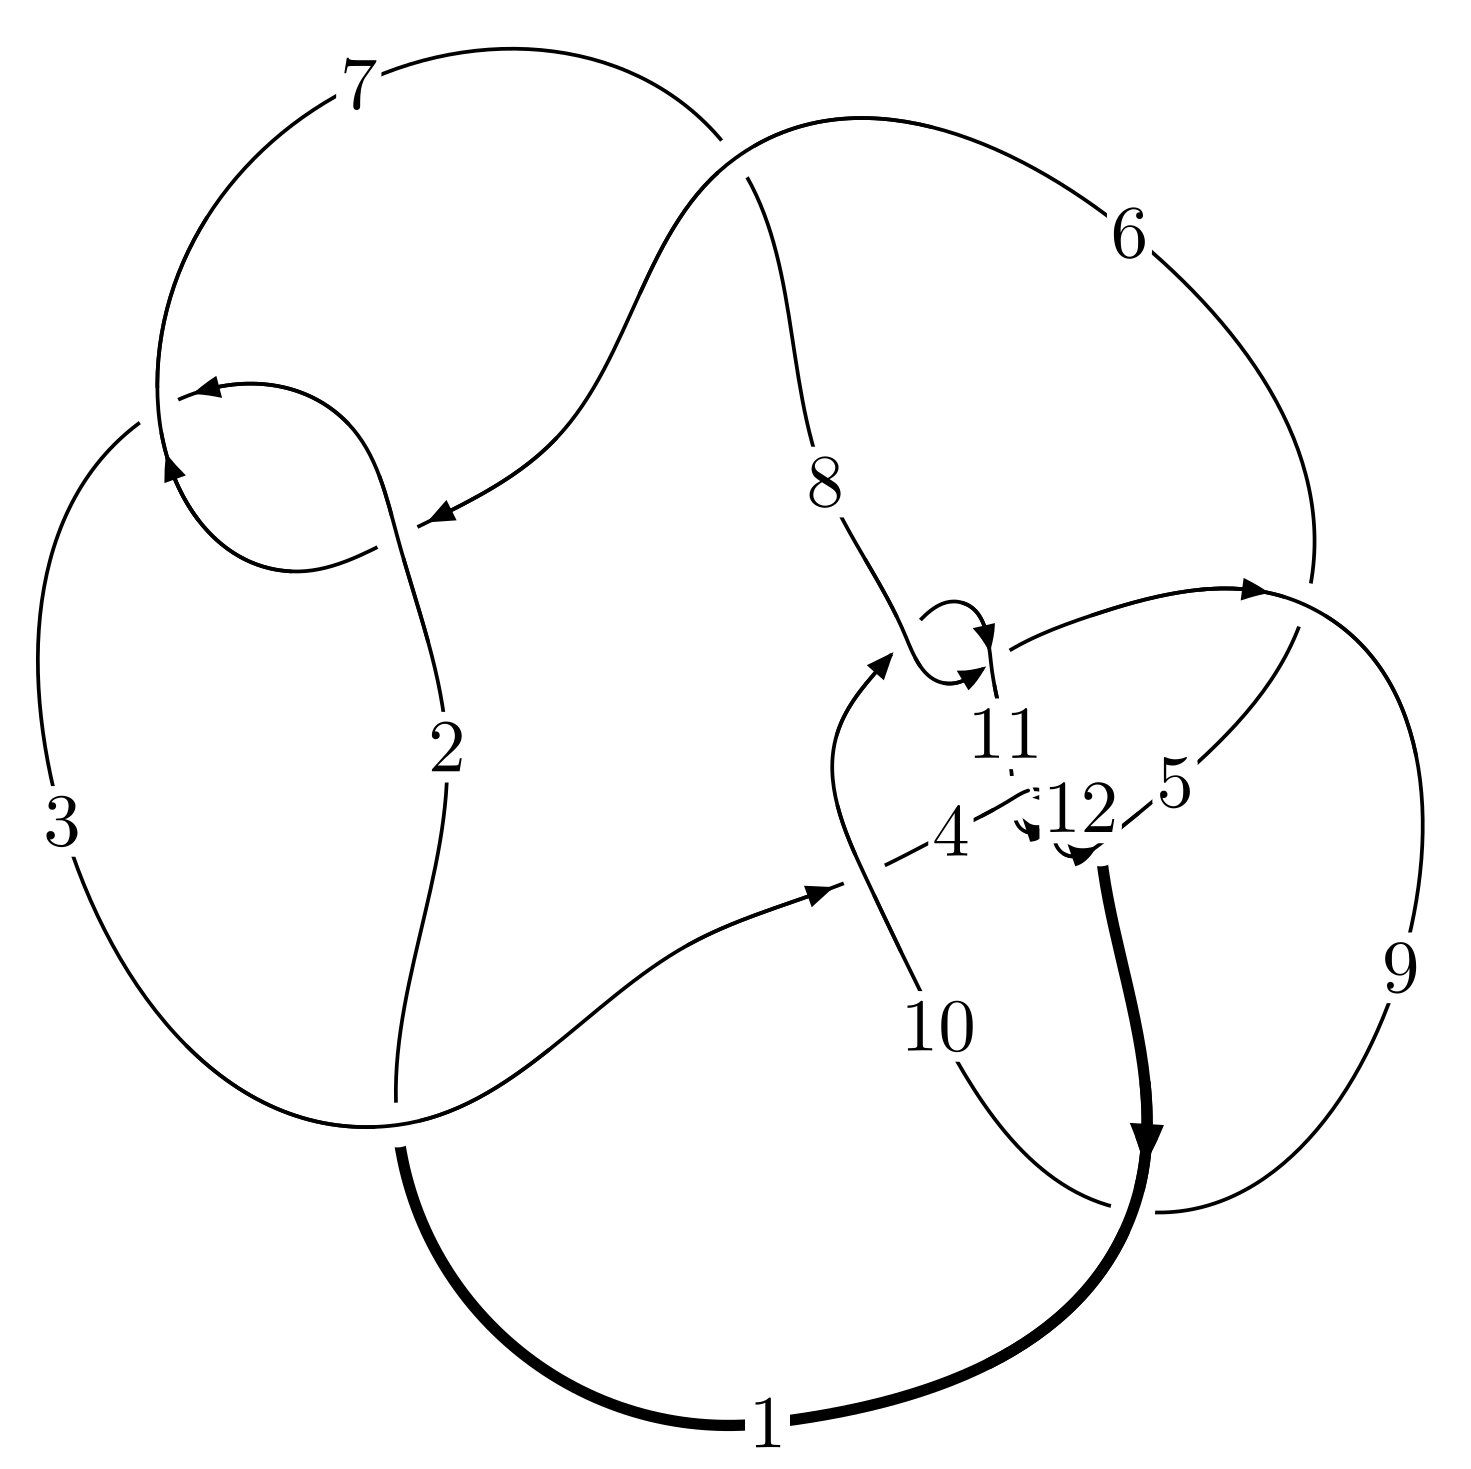
\includegraphics[width=112pt]{../../../GIT/diagram.site/Diagrams/png/1458_12a_0657.png}\\
\ \ \ A knot diagram\footnotemark}&
\allowdisplaybreaks
\textbf{Linearized knot diagam} \\
\cline{2-2}
 &
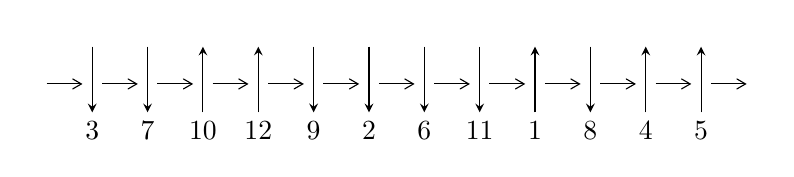
\begin{tikzpicture}[x=20pt, y=17pt]
	% nodes
	\node (C0) at (0, 0) {};
	\node (C1) at (1, 0) {};
	\node (C1U) at (1, +1) {};
	\node (C1D) at (1, -1) {3};

	\node (C2) at (2, 0) {};
	\node (C2U) at (2, +1) {};
	\node (C2D) at (2, -1) {7};

	\node (C3) at (3, 0) {};
	\node (C3U) at (3, +1) {};
	\node (C3D) at (3, -1) {10};

	\node (C4) at (4, 0) {};
	\node (C4U) at (4, +1) {};
	\node (C4D) at (4, -1) {12};

	\node (C5) at (5, 0) {};
	\node (C5U) at (5, +1) {};
	\node (C5D) at (5, -1) {9};

	\node (C6) at (6, 0) {};
	\node (C6U) at (6, +1) {};
	\node (C6D) at (6, -1) {2};

	\node (C7) at (7, 0) {};
	\node (C7U) at (7, +1) {};
	\node (C7D) at (7, -1) {6};

	\node (C8) at (8, 0) {};
	\node (C8U) at (8, +1) {};
	\node (C8D) at (8, -1) {11};

	\node (C9) at (9, 0) {};
	\node (C9U) at (9, +1) {};
	\node (C9D) at (9, -1) {1};

	\node (C10) at (10, 0) {};
	\node (C10U) at (10, +1) {};
	\node (C10D) at (10, -1) {8};

	\node (C11) at (11, 0) {};
	\node (C11U) at (11, +1) {};
	\node (C11D) at (11, -1) {4};

	\node (C12) at (12, 0) {};
	\node (C12U) at (12, +1) {};
	\node (C12D) at (12, -1) {5};
	\node (C13) at (13, 0) {};

	% arrows
	\draw[->,>={angle 60}]
	(C0) edge (C1) (C1) edge (C2) (C2) edge (C3) (C3) edge (C4) (C4) edge (C5) (C5) edge (C6) (C6) edge (C7) (C7) edge (C8) (C8) edge (C9) (C9) edge (C10) (C10) edge (C11) (C11) edge (C12) (C12) edge (C13) ;	\draw[->,>=stealth]
	(C1U) edge (C1D) (C2U) edge (C2D) (C3D) edge (C3U) (C4D) edge (C4U) (C5U) edge (C5D) (C6U) edge (C6D) (C7U) edge (C7D) (C8U) edge (C8D) (C9D) edge (C9U) (C10U) edge (C10D) (C11D) edge (C11U) (C12D) edge (C12U) ;
	\end{tikzpicture} \\
\hhline{~~} \\& 
\textbf{Solving Sequence} \\ \cline{2-2} 
 &
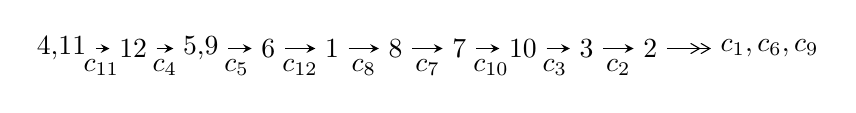
\begin{tikzpicture}[x=23pt, y=7pt]
	% node
	\node (A0) at (-1/8, 0) {4,11};
	\node (A1) at (1, 0) {12};
	\node (A2) at (33/16, 0) {5,9};
	\node (A3) at (25/8, 0) {6};
	\node (A4) at (33/8, 0) {1};
	\node (A5) at (41/8, 0) {8};
	\node (A6) at (49/8, 0) {7};
	\node (A7) at (57/8, 0) {10};
	\node (A8) at (65/8, 0) {3};
	\node (A9) at (73/8, 0) {2};
	\node (C1) at (1/2, -1) {$c_{11}$};
	\node (C2) at (3/2, -1) {$c_{4}$};
	\node (C3) at (21/8, -1) {$c_{5}$};
	\node (C4) at (29/8, -1) {$c_{12}$};
	\node (C5) at (37/8, -1) {$c_{8}$};
	\node (C6) at (45/8, -1) {$c_{7}$};
	\node (C7) at (53/8, -1) {$c_{10}$};
	\node (C8) at (61/8, -1) {$c_{3}$};
	\node (C9) at (69/8, -1) {$c_{2}$};
	\node (A10) at (11, 0) {$c_{1},c_{6},c_{9}$};

	% edge
	\draw[->,>=stealth]	
	(A0) edge (A1) (A1) edge (A2) (A2) edge (A3) (A3) edge (A4) (A4) edge (A5) (A5) edge (A6) (A6) edge (A7) (A7) edge (A8) (A8) edge (A9) ;
	\draw[->>,>={angle 60}]	
	(A9) edge (A10);
\end{tikzpicture} \\ 

\end{tabular} \\

\footnotetext{
The image of knot diagram is generated by the software ``\textbf{Draw programme}" developed by Andrew Bartholomew(\url{http://www.layer8.co.uk/maths/draw/index.htm\#Running-draw}), where we modified some parts for our purpose(\url{https://github.com/CATsTAILs/LinksPainter}).
}\phantom \\ \newline 
\centering \textbf{Ideals for irreducible components\footnotemark of $X_{\text{par}}$} 
 
\begin{align*}
I^u_{1}&=\langle 
2.50294\times10^{149} u^{95}+9.60419\times10^{149} u^{94}+\cdots+5.45085\times10^{150} b+7.14187\times10^{150},\\
\phantom{I^u_{1}}&\phantom{= \langle  }5.49450\times10^{151} u^{95}+1.92581\times10^{152} u^{94}+\cdots+1.25370\times10^{152} a-2.01529\times10^{152},\;u^{96}+2 u^{95}+\cdots+2 u^2+1\rangle \\
I^u_{2}&=\langle 
b+1,\;12 u^5+2 u^4-25 u^3+14 u^2+23 a+24 u-7,\;u^6- u^5- u^4+2 u^3- u+1\rangle \\
\\
\end{align*}
\raggedright * 2 irreducible components of $\dim_{\mathbb{C}}=0$, with total 102 representations.\\
\footnotetext{All coefficients of polynomials are rational numbers. But the coefficients are sometimes approximated in decimal forms when there is not enough margin.}
\newpage
\renewcommand{\arraystretch}{1}
\centering \section*{I. $I^u_{1}= \langle 2.50\times10^{149} u^{95}+9.60\times10^{149} u^{94}+\cdots+5.45\times10^{150} b+7.14\times10^{150},\;5.49\times10^{151} u^{95}+1.93\times10^{152} u^{94}+\cdots+1.25\times10^{152} a-2.02\times10^{152},\;u^{96}+2 u^{95}+\cdots+2 u^2+1 \rangle$}
\flushleft \textbf{(i) Arc colorings}\\
\begin{tabular}{m{7pt} m{180pt} m{7pt} m{180pt} }
\flushright $a_{4}=$&$\begin{pmatrix}0\\u\end{pmatrix}$ \\
\flushright $a_{11}=$&$\begin{pmatrix}1\\0\end{pmatrix}$ \\
\flushright $a_{12}=$&$\begin{pmatrix}1\\- u^2\end{pmatrix}$ \\
\flushright $a_{5}=$&$\begin{pmatrix}u\\- u^3+u\end{pmatrix}$ \\
\flushright $a_{9}=$&$\begin{pmatrix}-0.438264 u^{95}-1.53611 u^{94}+\cdots-15.8344 u+1.60748\\-0.0459183 u^{95}-0.176196 u^{94}+\cdots-1.02762 u-1.31023\end{pmatrix}$ \\
\flushright $a_{6}=$&$\begin{pmatrix}2.34511 u^{95}+4.53792 u^{94}+\cdots-4.30308 u+6.52258\\-0.404134 u^{95}-0.805885 u^{94}+\cdots+3.44265 u+0.468334\end{pmatrix}$ \\
\flushright $a_{1}=$&$\begin{pmatrix}- u^2+1\\u^4-2 u^2\end{pmatrix}$ \\
\flushright $a_{8}=$&$\begin{pmatrix}-0.484182 u^{95}-1.71230 u^{94}+\cdots-16.8620 u+0.297252\\-0.0459183 u^{95}-0.176196 u^{94}+\cdots-1.02762 u-1.31023\end{pmatrix}$ \\
\flushright $a_{7}=$&$\begin{pmatrix}-0.948773 u^{95}-2.17227 u^{94}+\cdots-8.96234 u-2.40244\\0.0561849 u^{95}-0.157085 u^{94}+\cdots-1.71285 u-1.05821\end{pmatrix}$ \\
\flushright $a_{10}=$&$\begin{pmatrix}-0.349694 u^{95}-1.34273 u^{94}+\cdots-15.8119 u+1.44566\\-0.0232900 u^{95}-0.115177 u^{94}+\cdots-0.862337 u-1.28587\end{pmatrix}$ \\
\flushright $a_{3}=$&$\begin{pmatrix}1.33753 u^{95}+2.83107 u^{94}+\cdots-9.96316 u+6.91198\\-0.555614 u^{95}-0.988189 u^{94}+\cdots+2.17596 u+0.0933008\end{pmatrix}$ \\
\flushright $a_{2}=$&$\begin{pmatrix}-0.0756936 u^{95}-0.257581 u^{94}+\cdots-8.23068 u+3.42725\\0.0319373 u^{95}+0.0106439 u^{94}+\cdots+0.274085 u-0.354842\end{pmatrix}$\\&\end{tabular}
\flushleft \textbf{(ii) Obstruction class $= -1$}\\~\\
\flushleft \textbf{(iii) Cusp Shapes $= 3.54301 u^{95}+5.85152 u^{94}+\cdots-26.2365 u+1.81413$}\\~\\
\newpage\renewcommand{\arraystretch}{1}
\flushleft \textbf{(iv) u-Polynomials at the component}\newline \\
\begin{tabular}{m{50pt}|m{274pt}}
Crossings & \hspace{64pt}u-Polynomials at each crossing \\
\hline $$\begin{aligned}c_{1},c_{7}\end{aligned}$$&$\begin{aligned}
&u^{96}+30 u^{95}+\cdots-4 u+1
\end{aligned}$\\
\hline $$\begin{aligned}c_{2},c_{6}\end{aligned}$$&$\begin{aligned}
&u^{96}-2 u^{95}+\cdots-2 u+1
\end{aligned}$\\
\hline $$\begin{aligned}c_{3}\end{aligned}$$&$\begin{aligned}
&23(23 u^{96}-123 u^{95}+\cdots-9356946 u+601141)
\end{aligned}$\\
\hline $$\begin{aligned}c_{4},c_{11},c_{12}\end{aligned}$$&$\begin{aligned}
&u^{96}-2 u^{95}+\cdots+2 u^2+1
\end{aligned}$\\
\hline $$\begin{aligned}c_{5}\end{aligned}$$&$\begin{aligned}
&23(23 u^{96}+8 u^{95}+\cdots-2521819 u+368999)
\end{aligned}$\\
\hline $$\begin{aligned}c_{8},c_{10}\end{aligned}$$&$\begin{aligned}
&u^{96}-7 u^{95}+\cdots-4077 u+529
\end{aligned}$\\
\hline $$\begin{aligned}c_{9}\end{aligned}$$&$\begin{aligned}
&u^{96}-7 u^{95}+\cdots-375360 u+33856
\end{aligned}$\\
\hline
\end{tabular}\\~\\
\newpage\renewcommand{\arraystretch}{1}
\flushleft \textbf{(v) Riley Polynomials at the component}\newline \\
\begin{tabular}{m{50pt}|m{274pt}}
Crossings & \hspace{64pt}Riley Polynomials at each crossing \\
\hline $$\begin{aligned}c_{1},c_{7}\end{aligned}$$&$\begin{aligned}
&y^{96}+74 y^{95}+\cdots+192 y+1
\end{aligned}$\\
\hline $$\begin{aligned}c_{2},c_{6}\end{aligned}$$&$\begin{aligned}
&y^{96}-30 y^{95}+\cdots+4 y+1
\end{aligned}$\\
\hline $$\begin{aligned}c_{3}\end{aligned}$$&$\begin{aligned}
&529\\
&\cdot(529 y^{96}-25893 y^{95}+\cdots-85531184791874 y+361370501881)
\end{aligned}$\\
\hline $$\begin{aligned}c_{4},c_{11},c_{12}\end{aligned}$$&$\begin{aligned}
&y^{96}-90 y^{95}+\cdots+4 y+1
\end{aligned}$\\
\hline $$\begin{aligned}c_{5}\end{aligned}$$&$\begin{aligned}
&529\\
&\cdot(529 y^{96}+8354 y^{95}+\cdots+6225987047943 y+136160262001)
\end{aligned}$\\
\hline $$\begin{aligned}c_{8},c_{10}\end{aligned}$$&$\begin{aligned}
&y^{96}-49 y^{95}+\cdots-6810037 y+279841
\end{aligned}$\\
\hline $$\begin{aligned}c_{9}\end{aligned}$$&$\begin{aligned}
&y^{96}-39 y^{95}+\cdots-23851958272 y+1146228736
\end{aligned}$\\
\hline
\end{tabular}\\~\\
\newpage\flushleft \textbf{(vi) Complex Volumes and Cusp Shapes}
$$\begin{array}{c|c|c}  
\text{Solutions to }I^u_{1}& \I (\text{vol} + \sqrt{-1}CS) & \text{Cusp shape}\\
 \hline 
\begin{aligned}
u &= \phantom{-}0.664093 + 0.724291 I \\
a &= -0.152601 + 0.267162 I \\
b &= \phantom{-}1.098560 + 0.527969 I\end{aligned}
 & \phantom{-}2.46810 - 8.40093 I & \phantom{-0.000000 } 0 \\ \hline\begin{aligned}
u &= \phantom{-}0.664093 - 0.724291 I \\
a &= -0.152601 - 0.267162 I \\
b &= \phantom{-}1.098560 - 0.527969 I\end{aligned}
 & \phantom{-}2.46810 + 8.40093 I & \phantom{-0.000000 } 0 \\ \hline\begin{aligned}
u &= \phantom{-}0.334101 + 0.923275 I \\
a &= \phantom{-}0.687547 + 0.470553 I \\
b &= \phantom{-}0.961263 - 0.266335 I\end{aligned}
 & -3.49169 - 0.00825 I & \phantom{-0.000000 } 0 \\ \hline\begin{aligned}
u &= \phantom{-}0.334101 - 0.923275 I \\
a &= \phantom{-}0.687547 - 0.470553 I \\
b &= \phantom{-}0.961263 + 0.266335 I\end{aligned}
 & -3.49169 + 0.00825 I & \phantom{-0.000000 } 0 \\ \hline\begin{aligned}
u &= -0.898631 + 0.504886 I \\
a &= \phantom{-}0.209912 - 0.192977 I \\
b &= \phantom{-}0.686280 - 0.190169 I\end{aligned}
 & \phantom{-}1.053310 - 0.710227 I & \phantom{-0.000000 } 0 \\ \hline\begin{aligned}
u &= -0.898631 - 0.504886 I \\
a &= \phantom{-}0.209912 + 0.192977 I \\
b &= \phantom{-}0.686280 + 0.190169 I\end{aligned}
 & \phantom{-}1.053310 + 0.710227 I & \phantom{-0.000000 } 0 \\ \hline\begin{aligned}
u &= -0.669520 + 0.697805 I \\
a &= -0.133986 - 0.212092 I \\
b &= \phantom{-}1.017990 - 0.549890 I\end{aligned}
 & \phantom{-}3.55019 + 2.39774 I & \phantom{-0.000000 } 0 \\ \hline\begin{aligned}
u &= -0.669520 - 0.697805 I \\
a &= -0.133986 + 0.212092 I \\
b &= \phantom{-}1.017990 + 0.549890 I\end{aligned}
 & \phantom{-}3.55019 - 2.39774 I & \phantom{-0.000000 } 0 \\ \hline\begin{aligned}
u &= \phantom{-}0.443174 + 0.848605 I \\
a &= \phantom{-}0.630015 + 0.813518 I \\
b &= \phantom{-}1.171900 - 0.445009 I\end{aligned}
 & -4.58322 + 7.44174 I & \phantom{-0.000000 } 0 \\ \hline\begin{aligned}
u &= \phantom{-}0.443174 - 0.848605 I \\
a &= \phantom{-}0.630015 - 0.813518 I \\
b &= \phantom{-}1.171900 + 0.445009 I\end{aligned}
 & -4.58322 - 7.44174 I & \phantom{-0.000000 } 0\\
 \hline 
 \end{array}$$\newpage$$\begin{array}{c|c|c}  
\text{Solutions to }I^u_{1}& \I (\text{vol} + \sqrt{-1}CS) & \text{Cusp shape}\\
 \hline 
\begin{aligned}
u &= \phantom{-}0.463645 + 0.806284 I \\
a &= \phantom{-}0.695610 + 1.020350 I \\
b &= \phantom{-}1.248500 - 0.622548 I\end{aligned}
 & \phantom{-}1.86564 + 13.55260 I & \phantom{-0.000000 } 0 \\ \hline\begin{aligned}
u &= \phantom{-}0.463645 - 0.806284 I \\
a &= \phantom{-}0.695610 - 1.020350 I \\
b &= \phantom{-}1.248500 + 0.622548 I\end{aligned}
 & \phantom{-}1.86564 - 13.55260 I & \phantom{-0.000000 } 0 \\ \hline\begin{aligned}
u &= -0.452945 + 0.802837 I \\
a &= \phantom{-}0.746322 - 0.987694 I \\
b &= \phantom{-}1.193980 + 0.629248 I\end{aligned}
 & \phantom{-}2.88022 - 7.47631 I & \phantom{-0.000000 } 0 \\ \hline\begin{aligned}
u &= -0.452945 - 0.802837 I \\
a &= \phantom{-}0.746322 + 0.987694 I \\
b &= \phantom{-}1.193980 - 0.629248 I\end{aligned}
 & \phantom{-}2.88022 + 7.47631 I & \phantom{-0.000000 } 0 \\ \hline\begin{aligned}
u &= -0.384282 + 0.833895 I \\
a &= \phantom{-}0.799115 - 0.692769 I \\
b &= \phantom{-}0.996785 + 0.458170 I\end{aligned}
 & -0.41962 - 4.20352 I & \phantom{-0.000000 } 0 \\ \hline\begin{aligned}
u &= -0.384282 - 0.833895 I \\
a &= \phantom{-}0.799115 + 0.692769 I \\
b &= \phantom{-}0.996785 - 0.458170 I\end{aligned}
 & -0.41962 + 4.20352 I & \phantom{-0.000000 } 0 \\ \hline\begin{aligned}
u &= \phantom{-}0.792963 + 0.739457 I \\
a &= \phantom{-}0.028708 + 0.283343 I \\
b &= \phantom{-}0.971436 + 0.287560 I\end{aligned}
 & -3.61912 - 2.02495 I & \phantom{-0.000000 } 0 \\ \hline\begin{aligned}
u &= \phantom{-}0.792963 - 0.739457 I \\
a &= \phantom{-}0.028708 - 0.283343 I \\
b &= \phantom{-}0.971436 - 0.287560 I\end{aligned}
 & -3.61912 + 2.02495 I & \phantom{-0.000000 } 0 \\ \hline\begin{aligned}
u &= -0.488518 + 0.562688 I \\
a &= -0.161461 + 0.365143 I \\
b &= \phantom{-}0.306469 - 1.012220 I\end{aligned}
 & \phantom{-}5.59468 - 1.63818 I & \phantom{-}2.91885 + 2.68562 I \\ \hline\begin{aligned}
u &= -0.488518 - 0.562688 I \\
a &= -0.161461 - 0.365143 I \\
b &= \phantom{-}0.306469 + 1.012220 I\end{aligned}
 & \phantom{-}5.59468 + 1.63818 I & \phantom{-}2.91885 - 2.68562 I\\
 \hline 
 \end{array}$$\newpage$$\begin{array}{c|c|c}  
\text{Solutions to }I^u_{1}& \I (\text{vol} + \sqrt{-1}CS) & \text{Cusp shape}\\
 \hline 
\begin{aligned}
u &= -0.322988 + 0.658130 I \\
a &= \phantom{-}1.37204 - 0.52486 I \\
b &= \phantom{-}0.498271 + 0.624414 I\end{aligned}
 & \phantom{-}5.05930 - 2.23755 I & \phantom{-}2.52582 + 5.05237 I \\ \hline\begin{aligned}
u &= -0.322988 - 0.658130 I \\
a &= \phantom{-}1.37204 + 0.52486 I \\
b &= \phantom{-}0.498271 - 0.624414 I\end{aligned}
 & \phantom{-}5.05930 + 2.23755 I & \phantom{-}2.52582 - 5.05237 I \\ \hline\begin{aligned}
u &= -1.26745\phantom{ +0.000000I} \\
a &= \phantom{-}1.06705\phantom{ +0.000000I} \\
b &= -1.64301\phantom{ +0.000000I}\end{aligned}
 & -1.61828\phantom{ +0.000000I} & \phantom{-0.000000 } 0 \\ \hline\begin{aligned}
u &= \phantom{-}0.466641 + 0.564477 I \\
a &= -0.178245 - 0.425650 I \\
b &= \phantom{-}0.225474 + 1.073180 I\end{aligned}
 & \phantom{-}5.01127 + 7.57568 I & \phantom{-}1.49767 - 8.14095 I \\ \hline\begin{aligned}
u &= \phantom{-}0.466641 - 0.564477 I \\
a &= -0.178245 + 0.425650 I \\
b &= \phantom{-}0.225474 - 1.073180 I\end{aligned}
 & \phantom{-}5.01127 - 7.57568 I & \phantom{-}1.49767 + 8.14095 I \\ \hline\begin{aligned}
u &= -1.268200 + 0.059476 I \\
a &= \phantom{-}1.18929 + 0.81468 I \\
b &= -1.65731 - 0.33248 I\end{aligned}
 & \phantom{-}2.12370 - 4.56403 I & \phantom{-0.000000 } 0 \\ \hline\begin{aligned}
u &= -1.268200 - 0.059476 I \\
a &= \phantom{-}1.18929 - 0.81468 I \\
b &= -1.65731 + 0.33248 I\end{aligned}
 & \phantom{-}2.12370 + 4.56403 I & \phantom{-0.000000 } 0 \\ \hline\begin{aligned}
u &= \phantom{-}1.096330 + 0.643778 I \\
a &= \phantom{-}0.158040 + 0.346095 I \\
b &= \phantom{-}0.837642 + 0.052188 I\end{aligned}
 & -1.26594 + 5.58854 I & \phantom{-0.000000 } 0 \\ \hline\begin{aligned}
u &= \phantom{-}1.096330 - 0.643778 I \\
a &= \phantom{-}0.158040 - 0.346095 I \\
b &= \phantom{-}0.837642 - 0.052188 I\end{aligned}
 & -1.26594 - 5.58854 I & \phantom{-0.000000 } 0 \\ \hline\begin{aligned}
u &= \phantom{-}1.290000 + 0.078493 I \\
a &= \phantom{-}1.01584 - 1.13931 I \\
b &= -1.53554 + 0.46369 I\end{aligned}
 & \phantom{-}2.40735 - 0.56323 I & \phantom{-0.000000 } 0\\
 \hline 
 \end{array}$$\newpage$$\begin{array}{c|c|c}  
\text{Solutions to }I^u_{1}& \I (\text{vol} + \sqrt{-1}CS) & \text{Cusp shape}\\
 \hline 
\begin{aligned}
u &= \phantom{-}1.290000 - 0.078493 I \\
a &= \phantom{-}1.01584 + 1.13931 I \\
b &= -1.53554 - 0.46369 I\end{aligned}
 & \phantom{-}2.40735 + 0.56323 I & \phantom{-0.000000 } 0 \\ \hline\begin{aligned}
u &= -0.609114 + 0.334240 I \\
a &= \phantom{-}0.318331 + 0.157551 I \\
b &= \phantom{-}0.287889 - 0.332864 I\end{aligned}
 & \phantom{-}1.146790 - 0.591982 I & \phantom{-}6.49485 + 1.54474 I \\ \hline\begin{aligned}
u &= -0.609114 - 0.334240 I \\
a &= \phantom{-}0.318331 - 0.157551 I \\
b &= \phantom{-}0.287889 + 0.332864 I\end{aligned}
 & \phantom{-}1.146790 + 0.591982 I & \phantom{-}6.49485 - 1.54474 I \\ \hline\begin{aligned}
u &= \phantom{-}0.321236 + 0.613505 I \\
a &= \phantom{-}1.49841 + 0.44718 I \\
b &= \phantom{-}0.363298 - 0.635825 I\end{aligned}
 & \phantom{-}4.61231 - 3.82498 I & \phantom{-}1.69669 + 0.30945 I \\ \hline\begin{aligned}
u &= \phantom{-}0.321236 - 0.613505 I \\
a &= \phantom{-}1.49841 - 0.44718 I \\
b &= \phantom{-}0.363298 + 0.635825 I\end{aligned}
 & \phantom{-}4.61231 + 3.82498 I & \phantom{-}1.69669 - 0.30945 I \\ \hline\begin{aligned}
u &= \phantom{-}1.338900 + 0.124894 I \\
a &= \phantom{-}0.78918 - 1.77567 I \\
b &= -1.18956 + 0.83118 I\end{aligned}
 & -0.06296 + 3.70917 I & \phantom{-0.000000 } 0 \\ \hline\begin{aligned}
u &= \phantom{-}1.338900 - 0.124894 I \\
a &= \phantom{-}0.78918 + 1.77567 I \\
b &= -1.18956 - 0.83118 I\end{aligned}
 & -0.06296 - 3.70917 I & \phantom{-0.000000 } 0 \\ \hline\begin{aligned}
u &= \phantom{-}1.353990 + 0.016673 I \\
a &= -0.834167 - 0.766801 I \\
b &= -1.168080 + 0.080602 I\end{aligned}
 & \phantom{-}1.89369 + 0.02531 I & \phantom{-0.000000 } 0 \\ \hline\begin{aligned}
u &= \phantom{-}1.353990 - 0.016673 I \\
a &= -0.834167 + 0.766801 I \\
b &= -1.168080 - 0.080602 I\end{aligned}
 & \phantom{-}1.89369 - 0.02531 I & \phantom{-0.000000 } 0 \\ \hline\begin{aligned}
u &= \phantom{-}1.360990 + 0.155619 I \\
a &= \phantom{-}0.63332 - 2.01476 I \\
b &= -0.98925 + 1.12317 I\end{aligned}
 & \phantom{-}4.77740 + 8.35511 I & \phantom{-0.000000 } 0\\
 \hline 
 \end{array}$$\newpage$$\begin{array}{c|c|c}  
\text{Solutions to }I^u_{1}& \I (\text{vol} + \sqrt{-1}CS) & \text{Cusp shape}\\
 \hline 
\begin{aligned}
u &= \phantom{-}1.360990 - 0.155619 I \\
a &= \phantom{-}0.63332 + 2.01476 I \\
b &= -0.98925 - 1.12317 I\end{aligned}
 & \phantom{-}4.77740 - 8.35511 I & \phantom{-0.000000 } 0 \\ \hline\begin{aligned}
u &= \phantom{-}0.417961 + 0.467588 I \\
a &= \phantom{-}0.077572 - 0.589308 I \\
b &= -0.094014 + 0.749714 I\end{aligned}
 & -1.06119 + 3.30659 I & -3.60035 - 9.06831 I \\ \hline\begin{aligned}
u &= \phantom{-}0.417961 - 0.467588 I \\
a &= \phantom{-}0.077572 + 0.589308 I \\
b &= -0.094014 - 0.749714 I\end{aligned}
 & -1.06119 - 3.30659 I & -3.60035 + 9.06831 I \\ \hline\begin{aligned}
u &= -1.370750 + 0.094332 I \\
a &= \phantom{-}0.58842 + 1.75045 I \\
b &= -0.938648 - 0.549645 I\end{aligned}
 & \phantom{-}3.04859 - 2.23764 I & \phantom{-0.000000 } 0 \\ \hline\begin{aligned}
u &= -1.370750 - 0.094332 I \\
a &= \phantom{-}0.58842 - 1.75045 I \\
b &= -0.938648 + 0.549645 I\end{aligned}
 & \phantom{-}3.04859 + 2.23764 I & \phantom{-0.000000 } 0 \\ \hline\begin{aligned}
u &= -1.373450 + 0.150990 I \\
a &= \phantom{-}0.54418 + 1.95382 I \\
b &= -0.863399 - 1.075360 I\end{aligned}
 & \phantom{-}5.36707 - 2.82780 I & \phantom{-0.000000 } 0 \\ \hline\begin{aligned}
u &= -1.373450 - 0.150990 I \\
a &= \phantom{-}0.54418 - 1.95382 I \\
b &= -0.863399 + 1.075360 I\end{aligned}
 & \phantom{-}5.36707 + 2.82780 I & \phantom{-0.000000 } 0 \\ \hline\begin{aligned}
u &= \phantom{-}1.41758 + 0.04983 I \\
a &= \phantom{-}2.13899 - 2.92262 I \\
b &= -0.820464 + 0.008321 I\end{aligned}
 & \phantom{-}6.72398 - 2.80070 I & \phantom{-0.000000 } 0 \\ \hline\begin{aligned}
u &= \phantom{-}1.41758 - 0.04983 I \\
a &= \phantom{-}2.13899 + 2.92262 I \\
b &= -0.820464 - 0.008321 I\end{aligned}
 & \phantom{-}6.72398 + 2.80070 I & \phantom{-0.000000 } 0 \\ \hline\begin{aligned}
u &= -1.41743 + 0.05890 I \\
a &= \phantom{-}1.89221 + 2.25946 I \\
b &= -0.735464 - 0.033098 I\end{aligned}
 & \phantom{-}6.92096 - 2.88647 I & \phantom{-0.000000 } 0\\
 \hline 
 \end{array}$$\newpage$$\begin{array}{c|c|c}  
\text{Solutions to }I^u_{1}& \I (\text{vol} + \sqrt{-1}CS) & \text{Cusp shape}\\
 \hline 
\begin{aligned}
u &= -1.41743 - 0.05890 I \\
a &= \phantom{-}1.89221 - 2.25946 I \\
b &= -0.735464 + 0.033098 I\end{aligned}
 & \phantom{-}6.92096 + 2.88647 I & \phantom{-0.000000 } 0 \\ \hline\begin{aligned}
u &= -0.196684 + 0.513849 I \\
a &= -0.354453 + 0.932054 I \\
b &= -1.132040 - 0.750035 I\end{aligned}
 & -0.11950 - 5.94878 I & -5.44478 + 9.17655 I \\ \hline\begin{aligned}
u &= -0.196684 - 0.513849 I \\
a &= -0.354453 - 0.932054 I \\
b &= -1.132040 + 0.750035 I\end{aligned}
 & -0.11950 + 5.94878 I & -5.44478 - 9.17655 I \\ \hline\begin{aligned}
u &= \phantom{-}0.221448 + 0.498623 I \\
a &= -0.290394 - 0.994151 I \\
b &= -0.989290 + 0.743082 I\end{aligned}
 & \phantom{-}0.333283 + 0.495333 I & -3.97583 - 3.89260 I \\ \hline\begin{aligned}
u &= \phantom{-}0.221448 - 0.498623 I \\
a &= -0.290394 + 0.994151 I \\
b &= -0.989290 - 0.743082 I\end{aligned}
 & \phantom{-}0.333283 - 0.495333 I & -3.97583 + 3.89260 I \\ \hline\begin{aligned}
u &= -1.42650 + 0.28467 I \\
a &= \phantom{-}0.487682 - 1.290430 I \\
b &= \phantom{-}0.798971 + 0.614933 I\end{aligned}
 & \phantom{-}10.09940 + 0.42622 I & \phantom{-0.000000 } 0 \\ \hline\begin{aligned}
u &= -1.42650 - 0.28467 I \\
a &= \phantom{-}0.487682 + 1.290430 I \\
b &= \phantom{-}0.798971 - 0.614933 I\end{aligned}
 & \phantom{-}10.09940 - 0.42622 I & \phantom{-0.000000 } 0 \\ \hline\begin{aligned}
u &= \phantom{-}1.44291 + 0.28759 I \\
a &= \phantom{-}0.39822 + 1.39202 I \\
b &= \phantom{-}0.868280 - 0.653053 I\end{aligned}
 & \phantom{-}10.67610 + 5.79876 I & \phantom{-0.000000 } 0 \\ \hline\begin{aligned}
u &= \phantom{-}1.44291 - 0.28759 I \\
a &= \phantom{-}0.39822 - 1.39202 I \\
b &= \phantom{-}0.868280 + 0.653053 I\end{aligned}
 & \phantom{-}10.67610 - 5.79876 I & \phantom{-0.000000 } 0 \\ \hline\begin{aligned}
u &= -1.46807 + 0.17113 I \\
a &= -0.31675 + 1.45982 I \\
b &= \phantom{-}0.153260 - 1.105640 I\end{aligned}
 & \phantom{-}5.08717 - 5.68044 I & \phantom{-0.000000 } 0\\
 \hline 
 \end{array}$$\newpage$$\begin{array}{c|c|c}  
\text{Solutions to }I^u_{1}& \I (\text{vol} + \sqrt{-1}CS) & \text{Cusp shape}\\
 \hline 
\begin{aligned}
u &= -1.46807 - 0.17113 I \\
a &= -0.31675 - 1.45982 I \\
b &= \phantom{-}0.153260 + 1.105640 I\end{aligned}
 & \phantom{-}5.08717 + 5.68044 I & \phantom{-0.000000 } 0 \\ \hline\begin{aligned}
u &= -1.47757 + 0.19945 I \\
a &= -0.69290 + 1.56154 I \\
b &= \phantom{-}0.382716 - 1.339380 I\end{aligned}
 & \phantom{-}11.3102 - 10.3824 I & \phantom{-0.000000 } 0 \\ \hline\begin{aligned}
u &= -1.47757 - 0.19945 I \\
a &= -0.69290 - 1.56154 I \\
b &= \phantom{-}0.382716 + 1.339380 I\end{aligned}
 & \phantom{-}11.3102 + 10.3824 I & \phantom{-0.000000 } 0 \\ \hline\begin{aligned}
u &= \phantom{-}1.48389 + 0.19736 I \\
a &= -0.71198 - 1.46988 I \\
b &= \phantom{-}0.433648 + 1.280640 I\end{aligned}
 & \phantom{-}11.98830 + 4.43121 I & \phantom{-0.000000 } 0 \\ \hline\begin{aligned}
u &= \phantom{-}1.48389 - 0.19736 I \\
a &= -0.71198 + 1.46988 I \\
b &= \phantom{-}0.433648 - 1.280640 I\end{aligned}
 & \phantom{-}11.98830 - 4.43121 I & \phantom{-0.000000 } 0 \\ \hline\begin{aligned}
u &= -0.019785 + 0.498386 I \\
a &= -0.867519 + 0.145622 I \\
b &= -1.51285 - 0.08023 I\end{aligned}
 & -1.45387 + 2.58739 I & -7.88342 - 2.89181 I \\ \hline\begin{aligned}
u &= -0.019785 - 0.498386 I \\
a &= -0.867519 - 0.145622 I \\
b &= -1.51285 + 0.08023 I\end{aligned}
 & -1.45387 - 2.58739 I & -7.88342 + 2.89181 I \\ \hline\begin{aligned}
u &= -0.122494 + 0.481151 I \\
a &= -0.714382 + 0.841174 I \\
b &= -1.290580 - 0.423315 I\end{aligned}
 & -4.60245 - 1.56147 I & -13.5432 + 4.6448 I \\ \hline\begin{aligned}
u &= -0.122494 - 0.481151 I \\
a &= -0.714382 - 0.841174 I \\
b &= -1.290580 + 0.423315 I\end{aligned}
 & -4.60245 + 1.56147 I & -13.5432 - 4.6448 I \\ \hline\begin{aligned}
u &= \phantom{-}1.49943 + 0.16275 I \\
a &= -0.427368 - 1.103110 I \\
b &= \phantom{-}0.385106 + 0.904863 I\end{aligned}
 & \phantom{-}7.94574 + 2.75539 I & \phantom{-0.000000 } 0\\
 \hline 
 \end{array}$$\newpage$$\begin{array}{c|c|c}  
\text{Solutions to }I^u_{1}& \I (\text{vol} + \sqrt{-1}CS) & \text{Cusp shape}\\
 \hline 
\begin{aligned}
u &= \phantom{-}1.49943 - 0.16275 I \\
a &= -0.427368 + 1.103110 I \\
b &= \phantom{-}0.385106 - 0.904863 I\end{aligned}
 & \phantom{-}7.94574 - 2.75539 I & \phantom{-0.000000 } 0 \\ \hline\begin{aligned}
u &= -1.48030 + 0.33222 I \\
a &= -0.065804 - 1.268560 I \\
b &= \phantom{-}1.099420 + 0.493860 I\end{aligned}
 & \phantom{-}2.38632 - 4.46773 I & \phantom{-0.000000 } 0 \\ \hline\begin{aligned}
u &= -1.48030 - 0.33222 I \\
a &= -0.065804 + 1.268560 I \\
b &= \phantom{-}1.099420 - 0.493860 I\end{aligned}
 & \phantom{-}2.38632 + 4.46773 I & \phantom{-0.000000 } 0 \\ \hline\begin{aligned}
u &= \phantom{-}1.48751 + 0.30794 I \\
a &= -0.06205 + 1.50463 I \\
b &= \phantom{-}1.144410 - 0.624455 I\end{aligned}
 & \phantom{-}5.64050 + 8.33802 I & \phantom{-0.000000 } 0 \\ \hline\begin{aligned}
u &= \phantom{-}1.48751 - 0.30794 I \\
a &= -0.06205 - 1.50463 I \\
b &= \phantom{-}1.144410 + 0.624455 I\end{aligned}
 & \phantom{-}5.64050 - 8.33802 I & \phantom{-0.000000 } 0 \\ \hline\begin{aligned}
u &= -1.51878 + 0.10601 I \\
a &= -0.095323 + 0.663397 I \\
b &= \phantom{-}0.339093 - 0.482819 I\end{aligned}
 & \phantom{-}4.59539 - 0.33868 I & \phantom{-0.000000 } 0 \\ \hline\begin{aligned}
u &= -1.51878 - 0.10601 I \\
a &= -0.095323 - 0.663397 I \\
b &= \phantom{-}0.339093 + 0.482819 I\end{aligned}
 & \phantom{-}4.59539 + 0.33868 I & \phantom{-0.000000 } 0 \\ \hline\begin{aligned}
u &= \phantom{-}1.50456 + 0.29310 I \\
a &= -0.20692 + 1.76757 I \\
b &= \phantom{-}1.27782 - 0.74165 I\end{aligned}
 & \phantom{-}9.2181 + 11.4691 I & \phantom{-0.000000 } 0 \\ \hline\begin{aligned}
u &= \phantom{-}1.50456 - 0.29310 I \\
a &= -0.20692 - 1.76757 I \\
b &= \phantom{-}1.27782 + 0.74165 I\end{aligned}
 & \phantom{-}9.2181 - 11.4691 I & \phantom{-0.000000 } 0 \\ \hline\begin{aligned}
u &= -1.50426 + 0.30859 I \\
a &= -0.25757 - 1.54880 I \\
b &= \phantom{-}1.261580 + 0.609340 I\end{aligned}
 & \phantom{-}1.71020 - 11.63330 I & \phantom{-0.000000 } 0\\
 \hline 
 \end{array}$$\newpage$$\begin{array}{c|c|c}  
\text{Solutions to }I^u_{1}& \I (\text{vol} + \sqrt{-1}CS) & \text{Cusp shape}\\
 \hline 
\begin{aligned}
u &= -1.50426 - 0.30859 I \\
a &= -0.25757 + 1.54880 I \\
b &= \phantom{-}1.261580 - 0.609340 I\end{aligned}
 & \phantom{-}1.71020 + 11.63330 I & \phantom{-0.000000 } 0 \\ \hline\begin{aligned}
u &= -1.50851 + 0.29342 I \\
a &= -0.27033 - 1.78274 I \\
b &= \phantom{-}1.31646 + 0.73734 I\end{aligned}
 & \phantom{-}8.2521 - 17.5605 I & \phantom{-0.000000 } 0 \\ \hline\begin{aligned}
u &= -1.50851 - 0.29342 I \\
a &= -0.27033 + 1.78274 I \\
b &= \phantom{-}1.31646 - 0.73734 I\end{aligned}
 & \phantom{-}8.2521 + 17.5605 I & \phantom{-0.000000 } 0 \\ \hline\begin{aligned}
u &= \phantom{-}0.388560 + 0.226499 I \\
a &= \phantom{-}3.47210 - 1.47453 I \\
b &= -0.939752 - 0.290967 I\end{aligned}
 & \phantom{-}1.28524 + 1.87668 I & \phantom{-}1.39389 - 10.00654 I \\ \hline\begin{aligned}
u &= \phantom{-}0.388560 - 0.226499 I \\
a &= \phantom{-}3.47210 + 1.47453 I \\
b &= -0.939752 + 0.290967 I\end{aligned}
 & \phantom{-}1.28524 - 1.87668 I & \phantom{-}1.39389 + 10.00654 I \\ \hline\begin{aligned}
u &= -0.405275 + 0.182370 I \\
a &= \phantom{-}4.00898 + 1.36668 I \\
b &= -1.040670 + 0.259813 I\end{aligned}
 & \phantom{-}1.05835 + 3.63480 I & \phantom{-}3.32848 + 4.63258 I \\ \hline\begin{aligned}
u &= -0.405275 - 0.182370 I \\
a &= \phantom{-}4.00898 - 1.36668 I \\
b &= -1.040670 - 0.259813 I\end{aligned}
 & \phantom{-}1.05835 - 3.63480 I & \phantom{-}3.32848 - 4.63258 I \\ \hline\begin{aligned}
u &= \phantom{-}0.259608 + 0.355711 I \\
a &= \phantom{-}1.36832 - 0.40634 I \\
b &= -0.162394 - 0.150466 I\end{aligned}
 & -1.35358 - 0.59802 I & -5.31839 - 0.10830 I \\ \hline\begin{aligned}
u &= \phantom{-}0.259608 - 0.355711 I \\
a &= \phantom{-}1.36832 + 0.40634 I \\
b &= -0.162394 + 0.150466 I\end{aligned}
 & -1.35358 + 0.59802 I & -5.31839 + 0.10830 I \\ \hline\begin{aligned}
u &= \phantom{-}1.55443 + 0.17460 I \\
a &= -0.699112 - 0.633690 I \\
b &= \phantom{-}0.760656 + 0.693747 I\end{aligned}
 & \phantom{-}11.00460 + 0.65235 I & \phantom{-0.000000 } 0\\
 \hline 
 \end{array}$$\newpage$$\begin{array}{c|c|c}  
\text{Solutions to }I^u_{1}& \I (\text{vol} + \sqrt{-1}CS) & \text{Cusp shape}\\
 \hline 
\begin{aligned}
u &= \phantom{-}1.55443 - 0.17460 I \\
a &= -0.699112 + 0.633690 I \\
b &= \phantom{-}0.760656 - 0.693747 I\end{aligned}
 & \phantom{-}11.00460 - 0.65235 I & \phantom{-0.000000 } 0 \\ \hline\begin{aligned}
u &= -1.57253 + 0.17459 I \\
a &= -0.702518 + 0.492334 I \\
b &= \phantom{-}0.820732 - 0.598566 I\end{aligned}
 & \phantom{-}10.03080 + 5.18475 I & \phantom{-0.000000 } 0 \\ \hline\begin{aligned}
u &= -1.57253 - 0.17459 I \\
a &= -0.702518 - 0.492334 I \\
b &= \phantom{-}0.820732 + 0.598566 I\end{aligned}
 & \phantom{-}10.03080 - 5.18475 I & \phantom{-0.000000 } 0 \\ \hline\begin{aligned}
u &= \phantom{-}0.149227 + 0.346264 I \\
a &= -1.08762 - 2.24547 I \\
b &= -0.988148 + 0.176860 I\end{aligned}
 & -1.76677 + 0.65508 I & -4.67837 + 0.58281 I \\ \hline\begin{aligned}
u &= \phantom{-}0.149227 - 0.346264 I \\
a &= -1.08762 + 2.24547 I \\
b &= -0.988148 - 0.176860 I\end{aligned}
 & -1.76677 - 0.65508 I & -4.67837 - 0.58281 I \\ \hline\begin{aligned}
u &= -0.325727\phantom{ +0.000000I} \\
a &= \phantom{-}6.87271\phantom{ +0.000000I} \\
b &= -1.07784\phantom{ +0.000000I}\end{aligned}
 & -3.07701\phantom{ +0.000000I} & \phantom{-}21.8700\phantom{ +0.000000I}\\
 \hline 
 \end{array}$$\newpage\newpage\renewcommand{\arraystretch}{1}
\centering \section*{II. $I^u_{2}= \langle b+1,\;12 u^5+2 u^4-25 u^3+14 u^2+23 a+24 u-7,\;u^6- u^5- u^4+2 u^3- u+1 \rangle$}
\flushleft \textbf{(i) Arc colorings}\\
\begin{tabular}{m{7pt} m{180pt} m{7pt} m{180pt} }
\flushright $a_{4}=$&$\begin{pmatrix}0\\u\end{pmatrix}$ \\
\flushright $a_{11}=$&$\begin{pmatrix}1\\0\end{pmatrix}$ \\
\flushright $a_{12}=$&$\begin{pmatrix}1\\- u^2\end{pmatrix}$ \\
\flushright $a_{5}=$&$\begin{pmatrix}u\\- u^3+u\end{pmatrix}$ \\
\flushright $a_{9}=$&$\begin{pmatrix}-0.521739 u^{5}-0.0869565 u^{4}+\cdots-1.04348 u+0.304348\\-1\end{pmatrix}$ \\
\flushright $a_{6}=$&$\begin{pmatrix}0.330813 u^{5}-0.0680529 u^{4}+\cdots+1.27032 u+0.238185\\-0.391304 u^{5}+0.434783 u^{4}+\cdots+1.21739 u+0.478261\end{pmatrix}$ \\
\flushright $a_{1}=$&$\begin{pmatrix}- u^2+1\\u^4-2 u^2\end{pmatrix}$ \\
\flushright $a_{8}=$&$\begin{pmatrix}-0.521739 u^{5}-0.0869565 u^{4}+\cdots-1.04348 u-0.695652\\-1\end{pmatrix}$ \\
\flushright $a_{7}=$&$\begin{pmatrix}-0.262760 u^{5}-1.09452 u^{4}+\cdots-0.568998 u-0.669187\\0.956522 u^{5}-1.17391 u^{4}+\cdots+0.913043 u-1.39130\end{pmatrix}$ \\
\flushright $a_{10}=$&$\begin{pmatrix}-0.521739 u^{5}-0.0869565 u^{4}+\cdots-1.04348 u+0.304348\\-1\end{pmatrix}$ \\
\flushright $a_{3}=$&$\begin{pmatrix}-0.0264650 u^{5}+0.285444 u^{4}+\cdots+0.338374 u+0.500945\\-0.608696 u^{5}+0.565217 u^{4}+\cdots+0.782609 u+0.521739\end{pmatrix}$ \\
\flushright $a_{2}=$&$\begin{pmatrix}0.219282 u^{5}-0.0793951 u^{4}+\cdots+0.482042 u+1.27788\\0.0434783 u^{5}+0.173913 u^{4}+\cdots+0.0869565 u+0.391304\end{pmatrix}$\\&\end{tabular}
\flushleft \textbf{(ii) Obstruction class $= 1$}\\~\\
\flushleft \textbf{(iii) Cusp Shapes $= \frac{1575}{529} u^5-\frac{1911}{529} u^4-\frac{2712}{529} u^3+\frac{1803}{529} u^2-\frac{300}{529} u-\frac{4156}{529}$}\\~\\
\newpage\renewcommand{\arraystretch}{1}
\flushleft \textbf{(iv) u-Polynomials at the component}\newline \\
\begin{tabular}{m{50pt}|m{274pt}}
Crossings & \hspace{64pt}u-Polynomials at each crossing \\
\hline $$\begin{aligned}c_{1}\end{aligned}$$&$\begin{aligned}
&u^6-3 u^5+5 u^4-4 u^3+2 u^2- u+1
\end{aligned}$\\
\hline $$\begin{aligned}c_{2},c_{4}\end{aligned}$$&$\begin{aligned}
&u^6+u^5- u^4-2 u^3+u+1
\end{aligned}$\\
\hline $$\begin{aligned}c_{3}\end{aligned}$$&$\begin{aligned}
&23(23 u^6+18 u^5+25 u^4+8 u^3+7 u^2+u+1)
\end{aligned}$\\
\hline $$\begin{aligned}c_{5}\end{aligned}$$&$\begin{aligned}
&23(23 u^6+5 u^5-17 u^4-10 u^3+3 u^2+4 u+1)
\end{aligned}$\\
\hline $$\begin{aligned}c_{6},c_{11},c_{12}\end{aligned}$$&$\begin{aligned}
&u^6- u^5- u^4+2 u^3- u+1
\end{aligned}$\\
\hline $$\begin{aligned}c_{7}\end{aligned}$$&$\begin{aligned}
&u^6+3 u^5+5 u^4+4 u^3+2 u^2+u+1
\end{aligned}$\\
\hline $$\begin{aligned}c_{8}\end{aligned}$$&$\begin{aligned}
&(u-1)^6
\end{aligned}$\\
\hline $$\begin{aligned}c_{9}\end{aligned}$$&$\begin{aligned}
&u^6
\end{aligned}$\\
\hline $$\begin{aligned}c_{10}\end{aligned}$$&$\begin{aligned}
&(u+1)^6
\end{aligned}$\\
\hline
\end{tabular}\\~\\
\newpage\renewcommand{\arraystretch}{1}
\flushleft \textbf{(v) Riley Polynomials at the component}\newline \\
\begin{tabular}{m{50pt}|m{274pt}}
Crossings & \hspace{64pt}Riley Polynomials at each crossing \\
\hline $$\begin{aligned}c_{1},c_{7}\end{aligned}$$&$\begin{aligned}
&y^6+y^5+5 y^4+6 y^2+3 y+1
\end{aligned}$\\
\hline $$\begin{aligned}c_{2},c_{4},c_{6}\\c_{11},c_{12}\end{aligned}$$&$\begin{aligned}
&y^6-3 y^5+5 y^4-4 y^3+2 y^2- y+1
\end{aligned}$\\
\hline $$\begin{aligned}c_{3}\end{aligned}$$&$\begin{aligned}
&529(529 y^6+826 y^5+659 y^4+296 y^3+83 y^2+13 y+1)
\end{aligned}$\\
\hline $$\begin{aligned}c_{5}\end{aligned}$$&$\begin{aligned}
&529(529 y^6-807 y^5+527 y^4-196 y^3+55 y^2-10 y+1)
\end{aligned}$\\
\hline $$\begin{aligned}c_{8},c_{10}\end{aligned}$$&$\begin{aligned}
&(y-1)^6
\end{aligned}$\\
\hline $$\begin{aligned}c_{9}\end{aligned}$$&$\begin{aligned}
&y^6
\end{aligned}$\\
\hline
\end{tabular}\\~\\
\newpage\flushleft \textbf{(vi) Complex Volumes and Cusp Shapes}
$$\begin{array}{c|c|c}  
\text{Solutions to }I^u_{2}& \I (\text{vol} + \sqrt{-1}CS) & \text{Cusp shape}\\
 \hline 
\begin{aligned}
u &= -1.002190 + 0.295542 I \\
a &= \phantom{-}0.029335 + 0.442893 I \\
b &= -1.00000\phantom{ +0.000000I}\end{aligned}
 & \phantom{-}0.245672 - 0.924305 I & -2.62482 + 0.97831 I \\ \hline\begin{aligned}
u &= -1.002190 - 0.295542 I \\
a &= \phantom{-}0.029335 - 0.442893 I \\
b &= -1.00000\phantom{ +0.000000I}\end{aligned}
 & \phantom{-}0.245672 + 0.924305 I & -2.62482 - 0.97831 I \\ \hline\begin{aligned}
u &= \phantom{-}0.428243 + 0.664531 I \\
a &= -0.538704 - 0.781014 I \\
b &= -1.00000\phantom{ +0.000000I}\end{aligned}
 & -3.53554 - 0.92430 I & -5.29043 + 1.37115 I \\ \hline\begin{aligned}
u &= \phantom{-}0.428243 - 0.664531 I \\
a &= -0.538704 + 0.781014 I \\
b &= -1.00000\phantom{ +0.000000I}\end{aligned}
 & -3.53554 + 0.92430 I & -5.29043 - 1.37115 I \\ \hline\begin{aligned}
u &= \phantom{-}1.073950 + 0.558752 I \\
a &= -0.012370 - 0.494977 I \\
b &= -1.00000\phantom{ +0.000000I}\end{aligned}
 & -1.64493 + 5.69302 I & -9.84656 - 7.30057 I \\ \hline\begin{aligned}
u &= \phantom{-}1.073950 - 0.558752 I \\
a &= -0.012370 + 0.494977 I \\
b &= -1.00000\phantom{ +0.000000I}\end{aligned}
 & -1.64493 - 5.69302 I & -9.84656 + 7.30057 I\\
 \hline 
 \end{array}$$\newpage
\newpage\renewcommand{\arraystretch}{1}
\centering \section*{ III. u-Polynomials}
\begin{tabular}{m{50pt}|m{274pt}}
Crossings & \hspace{64pt}u-Polynomials at each crossing \\
\hline $$\begin{aligned}c_{1}\end{aligned}$$&$\begin{aligned}
&(u^6-3 u^5+5 u^4-4 u^3+2 u^2- u+1)(u^{96}+30 u^{95}+\cdots-4 u+1)
\end{aligned}$\\
\hline $$\begin{aligned}c_{2}\end{aligned}$$&$\begin{aligned}
&(u^6+u^5- u^4-2 u^3+u+1)(u^{96}-2 u^{95}+\cdots-2 u+1)
\end{aligned}$\\
\hline $$\begin{aligned}c_{3}\end{aligned}$$&$\begin{aligned}
&529(23 u^6+18 u^5+25 u^4+8 u^3+7 u^2+u+1)\\
&\cdot(23 u^{96}-123 u^{95}+\cdots-9356946 u+601141)
\end{aligned}$\\
\hline $$\begin{aligned}c_{4}\end{aligned}$$&$\begin{aligned}
&(u^6+u^5- u^4-2 u^3+u+1)(u^{96}-2 u^{95}+\cdots+2 u^2+1)
\end{aligned}$\\
\hline $$\begin{aligned}c_{5}\end{aligned}$$&$\begin{aligned}
&529(23 u^6+5 u^5-17 u^4-10 u^3+3 u^2+4 u+1)\\
&\cdot(23 u^{96}+8 u^{95}+\cdots-2521819 u+368999)
\end{aligned}$\\
\hline $$\begin{aligned}c_{6}\end{aligned}$$&$\begin{aligned}
&(u^6- u^5- u^4+2 u^3- u+1)(u^{96}-2 u^{95}+\cdots-2 u+1)
\end{aligned}$\\
\hline $$\begin{aligned}c_{7}\end{aligned}$$&$\begin{aligned}
&(u^6+3 u^5+5 u^4+4 u^3+2 u^2+u+1)(u^{96}+30 u^{95}+\cdots-4 u+1)
\end{aligned}$\\
\hline $$\begin{aligned}c_{8}\end{aligned}$$&$\begin{aligned}
&((u-1)^6)(u^{96}-7 u^{95}+\cdots-4077 u+529)
\end{aligned}$\\
\hline $$\begin{aligned}c_{9}\end{aligned}$$&$\begin{aligned}
&u^6(u^{96}-7 u^{95}+\cdots-375360 u+33856)
\end{aligned}$\\
\hline $$\begin{aligned}c_{10}\end{aligned}$$&$\begin{aligned}
&((u+1)^6)(u^{96}-7 u^{95}+\cdots-4077 u+529)
\end{aligned}$\\
\hline $$\begin{aligned}c_{11},c_{12}\end{aligned}$$&$\begin{aligned}
&(u^6- u^5- u^4+2 u^3- u+1)(u^{96}-2 u^{95}+\cdots+2 u^2+1)
\end{aligned}$\\
\hline
\end{tabular}\newpage\renewcommand{\arraystretch}{1}
\centering \section*{ IV. Riley Polynomials}
\begin{tabular}{m{50pt}|m{274pt}}
Crossings & \hspace{64pt}Riley Polynomials at each crossing \\
\hline $$\begin{aligned}c_{1},c_{7}\end{aligned}$$&$\begin{aligned}
&(y^6+y^5+5 y^4+6 y^2+3 y+1)(y^{96}+74 y^{95}+\cdots+192 y+1)
\end{aligned}$\\
\hline $$\begin{aligned}c_{2},c_{6}\end{aligned}$$&$\begin{aligned}
&(y^6-3 y^5+5 y^4-4 y^3+2 y^2- y+1)(y^{96}-30 y^{95}+\cdots+4 y+1)
\end{aligned}$\\
\hline $$\begin{aligned}c_{3}\end{aligned}$$&$\begin{aligned}
&279841(529 y^6+826 y^5+659 y^4+296 y^3+83 y^2+13 y+1)\\
&\cdot(529 y^{96}-25893 y^{95}+\cdots-85531184791874 y+361370501881)
\end{aligned}$\\
\hline $$\begin{aligned}c_{4},c_{11},c_{12}\end{aligned}$$&$\begin{aligned}
&(y^6-3 y^5+5 y^4-4 y^3+2 y^2- y+1)(y^{96}-90 y^{95}+\cdots+4 y+1)
\end{aligned}$\\
\hline $$\begin{aligned}c_{5}\end{aligned}$$&$\begin{aligned}
&279841(529 y^6-807 y^5+527 y^4-196 y^3+55 y^2-10 y+1)\\
&\cdot(529 y^{96}+8354 y^{95}+\cdots+6225987047943 y+136160262001)
\end{aligned}$\\
\hline $$\begin{aligned}c_{8},c_{10}\end{aligned}$$&$\begin{aligned}
&((y-1)^6)(y^{96}-49 y^{95}+\cdots-6810037 y+279841)
\end{aligned}$\\
\hline $$\begin{aligned}c_{9}\end{aligned}$$&$\begin{aligned}
&y^6(y^{96}-39 y^{95}+\cdots-2.38520\times10^{10} y+1.14623\times10^{9})
\end{aligned}$\\
\hline
\end{tabular}
\vskip 2pc
\end{document}